% ---------- SECTION IV - FIDO2 & WebAuthn ----------

\section{Results}
\label{sec:results}

To answer the research question, the literature is analyzed for two main topics: usability and security.\\
While there is some amount of research regarding the usability of \ac{fido2}, literature regarding the preceding protocols \ac{u2f} and \ac{uaf} is also taken into account due to the similarity of the involved hardware and authentication flows.\\
The security part of this chapter is mainly based on evaluations of the proposed concepts and mechanisms, as there is not yet any research regarding the security of actual implementations of either hardware or protocols.

% ---- Subsection Usability ----
\subsection{Usability}
\label{subsec:usability}

To determine whether a new authentication concept is accepted by users, and could therefore replace passwords, the usability plays a significant role. Regular passwords have been the prevalent authentication mechanism since the 1960's \cite{mcmillan2012}, so people are very familiar with their usage. The concept of sending credentials, checking them, and granting access to the protected ressource is also very intuitive. Using a hardware token, or in case of internal authenticators only a system dialogue, is a radically different approach.\\
A good starting point to evaluate whether this hardware-dependent approach is suitable is the study conducted by Lang et al \cite{lang2017}. The authors analyzed the roll-out of hardware tokens for 50,000 employees of Google as a second factor. In comparison to other \ac{2fa} methods like \ac{totp}, they found using a security key to be significantly faster.\\
On the other hand, a more qualitative and in-depth study of Das et al (2018) showed major usability problems for participants without technical backgrounds, especially during the initial setup. They report that users had trouble finding the correct instructions and where not able to intuitively use the device, as they had not yet developed a mental model regarding the functionality of the keys. The authors also explicitly state that one of the major problems was that users still had to enter their passwords, leading to additional work and complexity without any perceived benefit \cite{das2018}. This factor becomes less of a problem when a \ac{fido2} token is used for passwordless authentication.\\
\\
The most important scientific work for this section is a recent study by Lyastani et al, published in 2020, that focuses on the usability of \ac{fido2} as a means of passwordless, \ac{1fa}. They conclude that participants rated logging in via \ac{fido2} and an external authenticator as more usable than standard passwords, and were able to show a higher acceptance than the latter \cite{lyastani2020}.\\
However, the authors also identified some challenges, of which the most important ones are listed below:

\begin{description}
    \item[Complex Setup] Especially the initial registration of the key was seen as a challenge by many participants, this corresponds with the findings of \cite{das2018}.
    \item[Requires Physical Device] Users criticized that they had to carry an authenticator, and that the absence of this devices effectively logs them out of the application, substantially limiting spontaneous use.
    \item[Support of Other Devices] Logging in on devices without any way to connect the authenticator (e.g. a tablet or public PC without USB-A ports or NFC) is impossible.
    \item[Account Recovery after Loss] If the security key gets lost or stolen, account recovery is much more complex than with passwords. The current recommendation is to register a second backup key with each account \cite{gomi2019}.
    \item[No Account Delegation] It is not possible to grant a trusted third party (e.g. a colleague) access to an account without giving away the hardware key.
\end{description}


% ---- Subsection Security ----
\subsection{Security}
\label{subsec:security}

From a security point of view we can mainly analyze the concepts behind the protocols in the \ac{fido2} framework, as there is not yet any research regarding actual protocol implementations or hardware. Therefore, this section is mainly based on the official documentation and first evaluations of security researches. Additionally, we will look mostly at using \ac{fido2} in the passwordless, single factor mode.\\
The main difference to standard passwords is the use of public-key cryptography instead of storing a shared secret. For every new application the authenticator generates a separate key pair, of which only the public key is stored within the \acp{rp} servers. This has two implications: First, different credentials are used for every service, which means accounts cannot be linked across services based on the key, and as the user has no influence on the key generation, there is no way to derive user information from the public key. Second, as no secret is stored on the RPs side, a credential leak has no effect - knowing the public key is of no use for taking over an account. In addition to that resilience against credential leaks, the public-key infrastructure also prevents against phishing. Even if, for example, a malicious website could forge a \ac{fido2} authentication challenge using stolen public keys, the challenge response can not be used to login to the real account.\\
In general, public-key infrastructures are considered very robust and mature, although their security depends on the algorithm and key length used.\\
\\
While the protocols and general authentication flow can be seen as very secure and less prone to various attacks than passwords, another big factor of the general security are the authenticators themselfs. In all cases, it should not be possible to extract the private keys from the authenticator. Additionally, the presence and consent of the user has to be determined for every login, meaning the person has to physically act by pressing a button or accepting a system dialog. This ensures that malicious services cannot trigger and sign assertions without the users knowledge. Many authenticators, like the popular YubiKey 5, also implement another factor like a \ac{pin} or a fingerprint sensor to further protect against theft \cite{yubikey_5_nfc,dunkelberger2018}.


% ---- Subsection Other ----
\subsection{Comparison}
\label{subsec:comparison}

The below comparison of passwords, FIDO2 passwordless login and FIDO U2F is based on the authentication method evaluation framework developed by Bonneau et al \cite{bonneau2012}. The evaluation of simple passwords, also proposed by the former authors and supported by others \cite{lyastani2020} is not changed.

\begin{figure*}[ht]
    \centering
    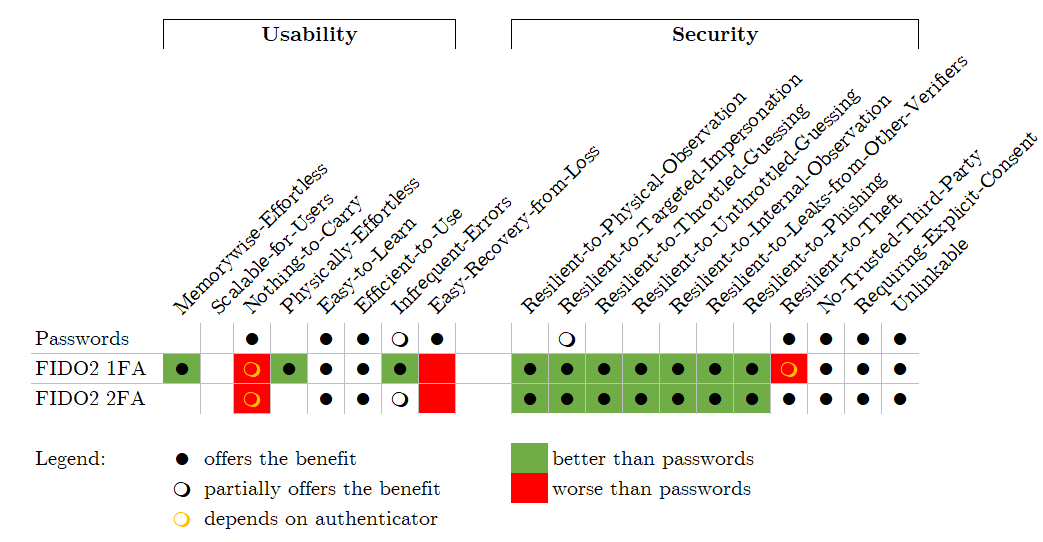
\includegraphics[width=1.8\columnwidth]{Figures/bonneau_matrix.png}
    \caption[Comparison of Authentication Methods]{Comparison of standard passwords with FIDO 1FA/2FA using a modified version of the framework proposed by Bonneau et al (2012)}
    \label{fig:bonneau_matrix}
\end{figure*}

\noindent As figure \ref{fig:bonneau_matrix} shows, both \ac{fido2} modes score exceptionally well. In fact, as is also mentioned in \cite{lyastani2020}, no other authentication method offers as many benefits as the former.